\subsection{Menambahkan Review}
    Halaman ini hanya dapat diakses oleh pengguna terdaftar yang sudah \textit{login}, dan hanya bisa menambahkan review kepada transaksi yang sudah selesai. Halaman ini menampilkan form \textit{modal} berisi \textit{input} data review, memberikan \textit{rating}. Pengguna dapat mengisi lalu mengklik tombol daftar, untuk kasus alternatif dapat dilihat pada Tabel \ref{uc04.02}.\\
	\indent Terdapat \textit{view logic} khusus dalam halaman ini, karena adanya proses pengecekan terlebih dahulu apakah pengguna sudah pernah memberi \textit{review} sebelumnya. Kode sumber implementasi \textit{back-end} dapat dilihat pada Kode Sumber \ref{cdbe.01-01}.

	\indent Tidak ada logika khusus, hanya logika \textit{back-end} ditulis menggunakan PHP yang dicantumkan dalam Kode Sumber \ref{cdbe.04-02};

\begin{figure}[H]
\centering
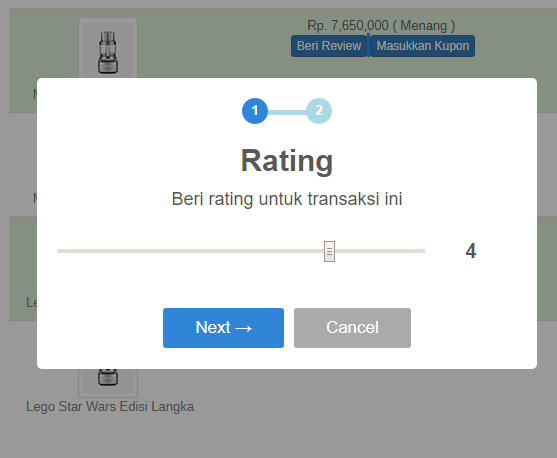
\includegraphics[width=\textwidth]{images/bab4/ui/04-02a.png}
\caption{Halaman Antarmuka Implementasi Menambahkan Review}
\label{ui.04-02a}
\end{figure}


\begin{figure}[H]
\centering
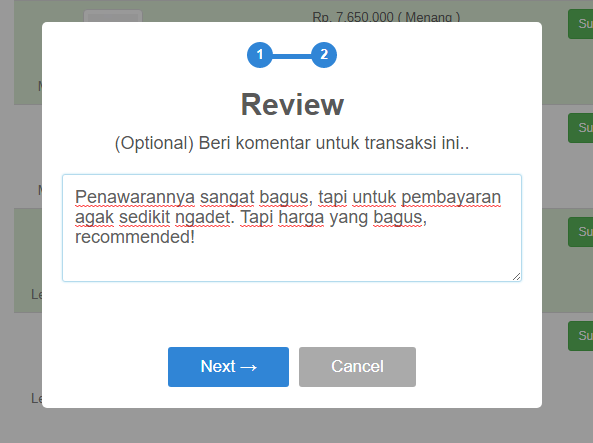
\includegraphics[width=\textwidth]{images/bab4/ui/04-02b.png}
\caption{Halaman Antarmuka Implementasi Menambahkan Review}
\label{ui.04-02b}
\end{figure}

\begin{lstlisting}[label=cdbe.04-02,style=php,caption=Kode Sumber \textit{Back-end} Menambahkan Review]
/*	file : app/Http/Controllers/ReviewController */
/* fungsi ini dieksekusi saat review disubmit */
    
public function submit(Request $request, $idbid)
{
    $informationNeeded = json_decode($request['info']);

    $bid = BidRepository::getBidDetail($idbid);
    $user = $request->user();
    if( !$bid || ($user->id != $bid->id_user && $user->id!= $bid->item->user->id) )
        abort(403);

    return response()
        ->json(
            ReviewRepository::submit($bid, $informationNeeded, $user)
        );
}

/*	file : app/Http/Controllers/ReviewRepository */
public static function submit(Bid $bid, $information, User $user)
{
    $constructArray = [
        'rate' => $information[0],
        'rate_message' => $information[1]
    ];

    $validator = Validator::make($constructArray, self::rule(), self::message());

    if ($validator->fails()) {
        return ['valid'=>false, 'msg'=> $validator->errors() ];
    }

    //stting user yang mau dirate as $user2
    if($user->id == $bid->id_user)
    {
        $user2 = $bid->item->user;
        $isBidder = true;
    }
    else if($user->id == $bid->item->user->id){
        $user2 = $bid->user;
        $isBidder = false;
    }

    $constructQuery = [
        'id_user_rater' => $user->id,
        'nama_user_rater' => $user->name,
        'rate' => $constructArray['rate'],
        'rate_message' => $constructArray['rate_message'],
        'id_item' => $bid->id_item,
        'bid_time' => $bid->bid_time
    ];

//        merge with

    if($isBidder)
        array_merge($constructQuery,
            ['id_user_auctioneer'=> $user2->id, 'nama_user_auctioneer' => $user2->name]);
    else
        array_merge($constructQuery,
            ['id_user_bidder'=> $user2->id, 'nama_user_bidder' => $user2->name]);

    $id = DB::table( $isBidder ? 'ratingauctioneers' : 'ratingbidders')
            ->insertGetId($constructQuery);

    if($id) return ['valid' => true];
        else return ['valid' => false, 'msg' => 'Maaf kesalahan server, silahkan coba lagi'];

    }

/*	file : app/Http/Controllers/BidRepository */
public static function getBidDetail($idbid){
    return Bid::findOrFail($idbid);
}



\end{lstlisting}